\chapter{Theoretischer Hintergrund}
Im folgenden Kapitel werden die theoretischen Grundlagen für diese Arbeit erläutert, um ein Verständnis für die verwendeten Begriffe und Technologien zu schaffen. Zunächst wird ein kurzer Überblick über die \ac{OCR} gegeben. Anschließend werden die Grundlagen der Transformer-Modelle erläutert. Des Weiteren werden die Details des \ac{Donut} genauer betrachtet, um ein Verständnis für die Funktionsweise des Modells im Vergleich zu herkömmlichen Methoden zu schaffen.

\section{Grundlagen der OCR}
Dieser Abschnitt betrachtet die grundlegende Funktionsweise und die Anwendungsbereiche von OCR-Systemen, da auch heute noch die meisten Modelle der Dokumentenverarbeitung auf eine OCR für den textuellen Input angewiesen sind (siehe dazu bspw. LayoutLM3\footcites[Vgl. dazu ausführlich][]{huang_layoutlmv3_2022}, ERNIE\footcites[Vgl. dazu ausführlich][]{peng_ernie-layout_2022}, FastStrucText\footcites[Vgl. dazu ausführlich][]{zhai_fast-structext_2023} etc.). Der Abschnitt bietet einen grundlegenden Überblick über das Thema. Auf ein tieferes Verständnis und eine detaillierte Betrachtung der Funktionsweise von OCR-Systemen wird in dieser Arbeit nicht eingegangen, da der Fokus auf der Anwendung von Transformer-Modellen im Bereich der Dokumentenverarbeitung liegt. Dennoch darf die Relevanz von OCR-Systemen nicht unterschätzt werden, da sie in vielen \ac{SOTA}-Modellen immer noch als Basis für die Textextraktion dienen. 

Häufig liegen Informationen in handschriftlicher oder gedruckter Form vor. Diese Informationen können durch Scans als Bilder in Computern gespeichert werden, jedoch ist die weiterverarbeitung der Informationen schwierig. Das System kann nicht ohne weiteres auf den Text in den erfassten Bildern zugreifen, bzw. diesen Lesen. Das Ziel von OCR ist es, Text aus Bildern zu extrahieren. OCR-Systeme sind in der Lage, Text aus gescannten Dokumenten, Fotos oder anderen Bildern zu extrahieren und in maschinenlesbaren Text umzuwandeln. In einem solchen Format können die Informationen weiterverarbeitet und analysiert werden. Somit ermöglicht es OCR einer Maschine, Texte automatisch zu erkennen.\footcites[Vgl.][S.244]{hamad_detailed_2016}

Für eine hohe Qualität und Genauigkeit der Zeichenerkennung erwarten OCR-Systeme eine hohe Qualität der Eingabebilder. Die Qualität der Eingabebilder ist ein entscheidender Punkt für die Genauigkeit der Zeichenerkennung. Einige Faktoren stellen Herausforderungen für die OCR dar, darunter die Szenenkomplexität, ungleiche Beleuchtungsbedingungen, Verzerrungen, Unschärfe und Abbau, Aspektverhältnisse, die Kippung, die Schriftart und mehrsprachige Umgebungen.\footcites[Vgl.][S.245]{hamad_detailed_2016} Die Herausforderungen erfordern fortgeschrittene Algorithmen und Techniken, einschließlich maschinellem Lernen und künstlicher Intelligenz, um die Erkennungsrate zu verbessern. Diese Herausforderungen versucht das Donut-Modell zu überwinden, indem es auf Transformer-Modellen basiert und somit die Limitierungen von OCR-Systemen umgeht.\footcites[Vgl.][S.1]{kim_ocr-free_2021} Um die Ergebnisse von OCR-Systemen zu verbessern werden in der Literatur verschiedene Ansätze vorgeschlagen. Nguyen et. al. schlagen die Verwendung von BERT vor. Als kontextbasiertes Sprachmodell kann BERT die Genauigkeit der OCR-Systeme verbessern, indem es die Kontextinformationen der Wörter berücksichtigt. Die Autoren zeigen, dass BERT die Genauigkeit der OCR-Systeme durch Fehlererkennung und Korrektur verbessern kann.\footcites[Vgl.][S.335 f.]{nguyen_neural_2020} BERT und seine Derivate werden noch heute in vielen \ac{SOTA}-Modellen für die Textextraktion verwendet.\footcites[Vgl. dazu ausführlich][S.4084 ff.]{huang_layoutlmv3_2022} \footcites[Vgl. dazu ausführlich][S.2 ff.]{garncarek_lambert_2020}

Die Funktionsweise von OCR-Systemen kann in sechs Phasen unterteilt werden. Diese Phasen umfassen die Vorverarbeitung, die Segmentierung, die Normalisierung, die Merkmalsextraktion, die Klassifikation und die Postverarbeitung. Das Ziel der Vorverarbeitung ist es, das Eingabebild zu verbessern und zu bereinigen. Die Segmentierung ist der Prozess, bei dem das Bild in einzelne Zeichen oder Wörter aufgeteilt und vom Hintergrund des Bildes getrennt wird. Sie stellt die kritische und maßgebliche Komponente eines OCR-Systems dar. Die Normalisierung ist der Prozess, bei dem die Segmentierungsergebnisse in eine standardisierte Form gebracht werden. In der Merkmalsextraktionsphase extrahiert das System relevante Merkmale von Objekten oder Alphabeten und wandelt diese zu Merkmalsvektoren um. In der Klassifikationsphase werden die Eingaben unterschiedlichen Klassen zugeordnet.\footcites[Vgl.][S.244]{hamad_detailed_2016} Beispielsweise wird in der Klassifikationsphase die Rechnungsnummer einer Klasse \emph{Invoice-Nr.} zugeordnet und das Datum der Klasse \emph{Date}. Es gibt diverse Werkzeuge, um die Klassifikation durchzuführen. Laut Dongre u.a. ist das \emph{Character Classification Problem} verwandt mit der heuristischen Logik, da Menschen Zeichen und Dokumente durch Erfahrung und Lernen erkennen können. Da Neuronale Netze ebenfalls von heuristischer Natur sind, sollten sie sich besonders gut für solche Probleme eignen. \footcites[Vgl.][S.11]{dongre_review_2010} Hier bleibt jedoch unbeachtet, dass die Eignung auch von der Qualität des Netzes selbst abhängt, welche wiederrum von der Qualität der Trainingsdaten abhängig ist.\footcites[Vgl.][S.851]{kavzoglu_increasing_2009} Daher eignet sich das Neuronale Netz als Klassifikator nur dann besonders gut, wenn die Trainingsdaten von hoher Qualität sind und das Netz in der Klassifikation eine hohe Genauigkeit aufweist. In der Postverarbeitung werden abschließend die Klassifikationsergebnisse weiterverarbeitet und korrigiert, um die Genauigkeit des erkannten Textes zu erhöhen.\footcites[Vgl.][S.246 f.]{hamad_detailed_2016} Hier wird das zuvor genannte BERT-Modell eingesetzt, um die Genauigkeit der OCR-Systeme zu verbessern.\footcites[Vgl.][S.335 f.]{nguyen_neural_2020}

Die Anwendungsbereiche der OCR sind vielfältig. Sie reichen von der Digitalisierung von Dokumenten in der Rechtsbranche über die Verarbeitung von Checks in Banken bis ins Gesundheitswesen. Der für diese Arbeit relevante Verwendungszweck ist die Verarbeitung von Rechnungen. OCR-Systeme werden in vielen Organisationen eingesetzt, um Rechnungen zu digitalisieren und diese so zu überwachen.\footcites[Vgl.][S.247 f.]{hamad_detailed_2016}

\section{Transformer-Modelle}
Im Folgenden soll ein Verständnis für die Transformer-Modelle geschaffen werden, welche wiederrum die Grundlage für Donut bilden. Dabei werden zunächst die Herkunft und Relevanz der Transformer-Modelle (folgend auch Transformer genannt) erläutert. Anschließend wird die Funktionsweise der Modelle genauer betrachtet. Dabei werden Schlüsselkonzepte wie die Aufmerksamkeit und das Positional Encoding, sowie die Architektur der Modelle erläutert. Seit der Einführung der Transformer in 2017 durch Vaswani et al. \footcites{vaswani_attention_2017} sind diese zum de facto Standard für eine Reihe verschiedener \ac{NLP} Aufgaben geworden. \ac{NLP} ist ein Teilbereich der Informatik, welcher es ermöglchen soll Computer Sprache auf eine \emph{natürliche} Art und Weise zu verstehen, so wie Menschen. Typischerweise refferenziert dies Aufgaben wie das Verstehen von Gefühlen in Texten, die Spracherkennung und das generieren von Antworten auf Fragen. \footcites[Vgl.][S.1]{beysolow_ii_applied_2018} Mittlerweile werden Transformer in den bekanntesten und meist genutzen Modellen der Welt verwendet, darunter BERT und GPT. \footcites[Vgl.][S. 1]{tunstall_natural_2022} Die beachtliche Leistungsfähigkeit der Transformer zeigt sich in den Benutzerzahlen von ChatGPT (ein ChatBot von OpenAI welcher auf den Transformer-Modellen basiert). Innerhalb von fünf Tage nach der Veröffentlichung des Modells hatte ChatGPT bereits eine Millionen Nutzer. Im Vergleich dazu brauchte Instagram zwei und halb Monate, um die gleiche Anzahl an Nutzern zu erreichen. \footcites[Vgl.][]{buchholz_infographic_2023} Den Status quo, vor der Entwicklung der Transformer, bildeten die \ac{RNN} und \ac{LSTM} Modelle. Transformer erzielen sowohl in der Leistungsfähigkeit als auch in den Trainingskosten bessere Ergebnisse als seine Vorgänger. \footcites[Vgl.][S. 1]{tunstall_natural_2022}

\subsection{Konzepte und Terminologie der Transformer-Modelle}

\subsection{Encoder-Decoder Architektur}
Das ursprüngliche Transformer-Modell, präsentiert von Vaswani et al. in 2017, basiert auf einer \emph{Encoder-Decoder} Architektur. Diese Architektur eignet sich besonder gut für Situationen, in welchen es sich sowohl bei der Ein- als auch der Ausgabe um Sequenzen handelt. Der Encoder wandelt die Eingabe von einer Sequenz in eine numerische Repräsentation um, welche häufig als \emph{last hidden state} bezeichnet wird. Dieser Zustand wird dann in den Decoder übergeben, welcher die Ausgabesequenz generiert. \footcites[Vgl.][S. 3]{tunstall_natural_2022}.

Der Aufbau der Encoder-Schicht kann Abb. \ref{fig:encoder-block} entnommen werden. Der Text wird zunächst in sog. \emph{Token Embeddings} umgewandelt. Das Ziel der Token Embeddings ist es Wörter, welche in Tokens umgewandelt wurden, in ihrem Kontext zu repräsentieren, da Wörter in verschiedenen Kontexten unterschiedliche Bedeutungen haben können. \footcites[Vgl.][S.692]{popa_towards_2021} %FIXME: Quelle selbst sagt Seite 2 aber das Magazin sagt 692...
Die Token Embeddings werden dann um \emph{Positional Embeddings} ergänzt. Diese repräsentieren die Position eines Tokens in einem Satz. Die Embeddings werden in den Encoder eingespeist, welcher die Eingabe in eine numerische Repräsentation umwandelt. Die Rolle des Encoders ist es die eingegangen Embeddings zu aktualisieren. Es sollen Repräsentationen von Tokens produziert werden, welche um kontextuelle Informationen angereichert sind. Beispielsweise wird das Wort \emph{Apple} aktualisiert, sodass es in einem unternehmerischen Kontext verstanden wird, wenn die Worte \emph{keynote} und \emph{phone} sich in der Nähe befinden. Konkret laufen die Embeddings durch zwei Schichten eines Encoder-Blocks: \footcites[Vgl.][S.58 ff.]{tunstall_natural_2022}
\begin{itemize}
    \item \emph{Multi-Head Attention Layer}
    \item \emph{Feed-Forward Layer}
\end{itemize}

\begin{figure}[h]
    \centering
    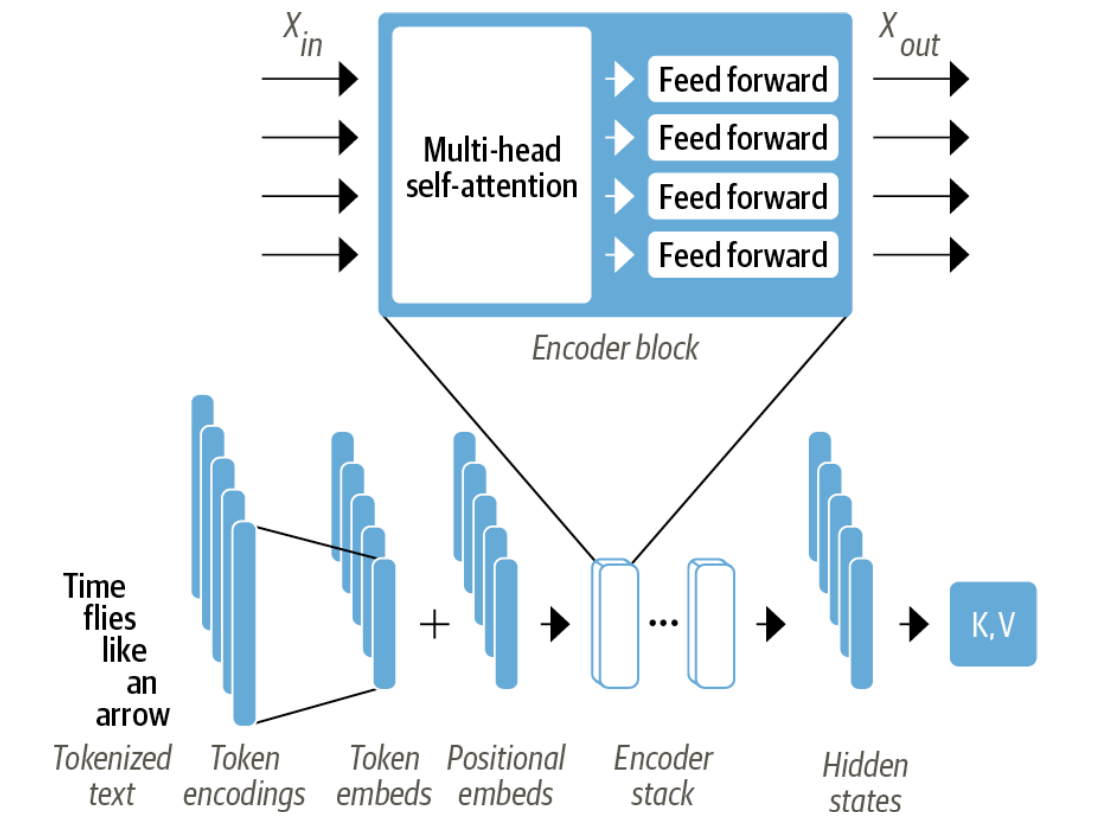
\includegraphics[height=80mm]{graphics/encoder-block.png}
    \caption[Aufbau eines Encoder-Blocks]{Aufbau eines Encoder-Blocks \footnotemark}
    \label{fig:encoder-block}
\end{figure}
\footnotetext{Entnommen aus: \cite{tunstall_natural_2022}, S.60}

